%!TeX encoding = UTF-8
%!TeX program = xelatex
\documentclass[notheorems, aspectratio=54]{beamer}
% aspectratio: 1610, 149, 54, 43(default), 32

\usepackage{latexsym}
\usepackage{amsmath,amssymb}
\usepackage{mathtools}
\usepackage{color,xcolor}
\usepackage{graphicx}
\usepackage{algorithm}
\usepackage{amsthm}
\usepackage{lmodern} % 解决 font warning
\usepackage[UTF8]{ctex}
\usepackage{animate} % insert gif

\usepackage{lipsum} % To generate test text 
\usepackage{ulem} % 下划线,波浪线

\usepackage{listings} % display code on slides; don't forget [fragile] option after \begin{frame}

% ----------------------------------------------
% tikx
\usepackage{framed}
\usepackage{tikz}
\usepackage{pgf}
\usetikzlibrary{calc,trees,positioning,arrows,chains,shapes.geometric,%
    decorations.pathreplacing,decorations.pathmorphing,shapes,%
    matrix,shapes.symbols}
\pgfmathsetseed{1} % To have predictable results
% Define a background layer, in which the parchment shape is drawn
\pgfdeclarelayer{background}
\pgfsetlayers{background,main}

% define styles for the normal border and the torn border
\tikzset{
  normal border/.style={orange!30!black!10, decorate, 
     decoration={random steps, segment length=2.5cm, amplitude=.7mm}},
  torn border/.style={orange!30!black!5, decorate, 
     decoration={random steps, segment length=.5cm, amplitude=1.7mm}}}

% Macro to draw the shape behind the text, when it fits completly in the
% page
\def\parchmentframe#1{
\tikz{
  \node[inner sep=2em] (A) {#1};  % Draw the text of the node
  \begin{pgfonlayer}{background}  % Draw the shape behind
  \fill[normal border] 
        (A.south east) -- (A.south west) -- 
        (A.north west) -- (A.north east) -- cycle;
  \end{pgfonlayer}}}

% Macro to draw the shape, when the text will continue in next page
\def\parchmentframetop#1{
\tikz{
  \node[inner sep=2em] (A) {#1};    % Draw the text of the node
  \begin{pgfonlayer}{background}    
  \fill[normal border]              % Draw the ``complete shape'' behind
        (A.south east) -- (A.south west) -- 
        (A.north west) -- (A.north east) -- cycle;
  \fill[torn border]                % Add the torn lower border
        ($(A.south east)-(0,.2)$) -- ($(A.south west)-(0,.2)$) -- 
        ($(A.south west)+(0,.2)$) -- ($(A.south east)+(0,.2)$) -- cycle;
  \end{pgfonlayer}}}

% Macro to draw the shape, when the text continues from previous page
\def\parchmentframebottom#1{
\tikz{
  \node[inner sep=2em] (A) {#1};   % Draw the text of the node
  \begin{pgfonlayer}{background}   
  \fill[normal border]             % Draw the ``complete shape'' behind
        (A.south east) -- (A.south west) -- 
        (A.north west) -- (A.north east) -- cycle;
  \fill[torn border]               % Add the torn upper border
        ($(A.north east)-(0,.2)$) -- ($(A.north west)-(0,.2)$) -- 
        ($(A.north west)+(0,.2)$) -- ($(A.north east)+(0,.2)$) -- cycle;
  \end{pgfonlayer}}}

% Macro to draw the shape, when both the text continues from previous page
% and it will continue in next page
\def\parchmentframemiddle#1{
\tikz{
  \node[inner sep=2em] (A) {#1};   % Draw the text of the node
  \begin{pgfonlayer}{background}   
  \fill[normal border]             % Draw the ``complete shape'' behind
        (A.south east) -- (A.south west) -- 
        (A.north west) -- (A.north east) -- cycle;
  \fill[torn border]               % Add the torn lower border
        ($(A.south east)-(0,.2)$) -- ($(A.south west)-(0,.2)$) -- 
        ($(A.south west)+(0,.2)$) -- ($(A.south east)+(0,.2)$) -- cycle;
  \fill[torn border]               % Add the torn upper border
        ($(A.north east)-(0,.2)$) -- ($(A.north west)-(0,.2)$) -- 
        ($(A.north west)+(0,.2)$) -- ($(A.north east)+(0,.2)$) -- cycle;
  \end{pgfonlayer}}}

% Define the environment which puts the frame
% In this case, the environment also accepts an argument with an optional
% title (which defaults to ``Example'', which is typeset in a box overlaid
% on the top border
\newenvironment{parchment}[1][Example]{%
  \def\FrameCommand{\parchmentframe}%
  \def\FirstFrameCommand{\parchmentframetop}%
  \def\LastFrameCommand{\parchmentframebottom}%
  \def\MidFrameCommand{\parchmentframemiddle}%
  \vskip\baselineskip
  \MakeFramed {\FrameRestore}
  \noindent\tikz\node[inner sep=1ex, draw=black!20,fill=white, 
          anchor=west, overlay] at (0em, 2em) {\sffamily#1};\par}%
{\endMakeFramed}

% ----------------------------------------------

\mode<presentation>{
    \usetheme{CambridgeUS}
    % Boadilla CambridgeUS
    % default Antibes Berlin Copenhagen
    % Madrid Montpelier Ilmenau Malmoe
    % Berkeley Singapore Warsaw
    \usecolortheme{beaver}
    % beetle, beaver, orchid, whale, dolphin
    \useoutertheme{infolines}
    % infolines miniframes shadow sidebar smoothbars smoothtree split tree
    \useinnertheme{circles}
    % circles, rectanges, rounded, inmargin
}
% 设置 block 颜色
\setbeamercolor{block title}{bg=red!30,fg=white}

\newcommand{\reditem}[1]{\setbeamercolor{item}{fg=red}\item #1}

% 缩放公式大小
\newcommand*{\Scale}[2][4]{\scalebox{#1}{\ensuremath{#2}}}

% 解决 font warning
\renewcommand\textbullet{\ensuremath{\bullet}}

% ---------------------------------------------------------------------
% flow chart
\tikzset{
    >=stealth',
    punktchain/.style={
        rectangle, 
        rounded corners, 
        % fill=black!10,
        draw=white, very thick,
        text width=6em,
        minimum height=2em, 
        text centered, 
        on chain
    },
    largepunktchain/.style={
        rectangle,
        rounded corners,
        draw=white, very thick,
        text width=10em,
        minimum height=2em,
        on chain
    },
    line/.style={draw, thick, <-},
    element/.style={
        tape,
        top color=white,
        bottom color=blue!50!black!60!,
        minimum width=6em,
        draw=blue!40!black!90, very thick,
        text width=6em, 
        minimum height=2em, 
        text centered, 
        on chain
    },
    every join/.style={->, thick,shorten >=1pt},
    decoration={brace},
    tuborg/.style={decorate},
    tubnode/.style={midway, right=2pt},
    font={\fontsize{10pt}{12}\selectfont},
}
% ---------------------------------------------------------------------

% code setting
\lstset{
    language=C++,
    basicstyle=\ttfamily\footnotesize,
    keywordstyle=\color{red},
    breaklines=true,
    xleftmargin=2em,
    numbers=left,
    numberstyle=\color[RGB]{222,155,81},
    frame=leftline,
    tabsize=4,
    breakatwhitespace=false,
    showspaces=false,               
    showstringspaces=false,
    showtabs=false,
    morekeywords={Str, Num, List},
}

% ---------------------------------------------------------------------

%% preamble
\title[Hog Binary Classifier]{Hog Binary Classifier}
% \subtitle{The subtitle}
\author{Internship Group 3}
\institute[]{Wang PuLi, Zhang Ling, Zheng Hui}

% -------------------------------------------------------------

\begin{document}

%% title frame
\begin{frame}
    \titlepage
\end{frame}

%% normal frame
\section{}
\subsection{}
% content frame
\begin{frame}
\frametitle{任务分工}
\begin{columns}
\begin{column}{.8\linewidth}
\begin{itemize}
	\item 张令: 数据预处理和数据标定.
	\item 王普莉: Binary Classifier编写和ROC曲线绘制.
	\item 郑晖: Hog算法实现.
	\item 全部代码可见: {\href{https://github.com/Fassial/zju-intern}{https://github.com/Fassial/zju-intern}}
\end{itemize}
\end{column}
\begin{column}{.2\linewidth}
\begin{figure}[htbp]
	\centering
	
\includegraphics[width=0.6\textwidth]{github.jpg}
\end{figure}
\end{column}
\end{columns}
\end{frame}

\begin{frame}
\frametitle{数据预处理和数据标定}
\begin{columns}
\begin{column}{.7\linewidth}
\begin{itemize}
	\item 框选篮筐部分
	\begin{itemize}
		\item recs1 = [880,90,960,170]
		\item recs2 = [945,230,1025,310]
		\item recs3 = [660,100,740,180]
	\end{itemize}
	\item 按帧分割为小图并作手工标定
	\begin{itemize}
		\item 按minute\_second\_frame的文件名格式分别保存在文件夹中。
		\item 挑选正样本集放到新文件夹real下。
	\end{itemize}
	\item 缩放为40*40像素并合并为大图
	\begin{itemize}
		\item 每一行存放1分钟内的60*25张子图。
		\item 将对应的label列表存入到npy文件中。
	\end{itemize}
	\item 编写My\_Explorers类,用于加载并访问数据集和标签
\end{itemize}
\end{column}
\begin{column}{.3\linewidth}
\begin{figure}[htbp]
	\centering
	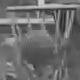
\includegraphics[width=0.6\textwidth]{goal.jpg}
\end{figure}
\end{column}
\end{columns}
\end{frame}

\begin{frame}
\frametitle{数据预处理和数据标定}
\begin{figure}[htbp]
	\centering
	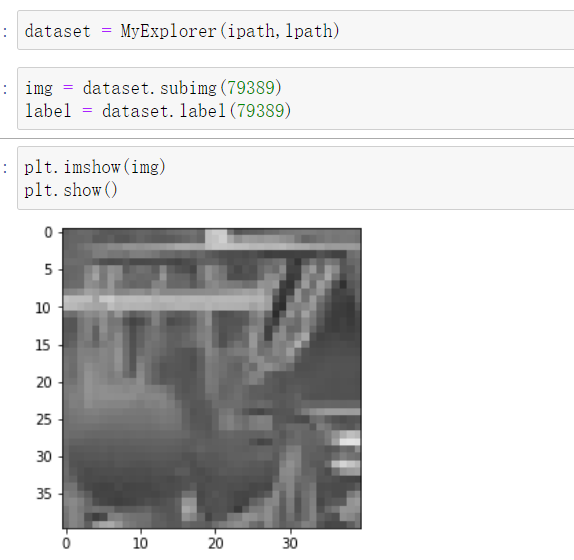
\includegraphics[width=0.6\textwidth]{myExplorer.png}
\end{figure}
\end{frame}

\begin{frame}
\frametitle{Binary Classifier编写和ROC曲线绘制}
\begin{columns}
\begin{column}{.5\linewidth}
\begin{itemize}
	\item get\_data
	\begin{itemize}
		\item 功能:提供加载数据的函数。
		\item 包含函数:read\_image。
	\end{itemize}
	\item binary\_classification
	\begin{itemize}
		\item 功能:提供用于训练、测试、画图的函数。
		\item 包含函数:get\_hog、threshold\_classifier、get\_roc\_data、draw\_roc\_data等。
	\end{itemize}
	\item config.ini
	\begin{itemize}
		\item 功能:配置文件,包含加载路径和ROC曲线保存的路径。
	\end{itemize}
	\item main
	\begin{itemize}
		\item 功能:主程序。
	\end{itemize}
\end{itemize}
\end{column}
\begin{column}{.5\linewidth}
\begin{figure}[htbp]
	\centering
	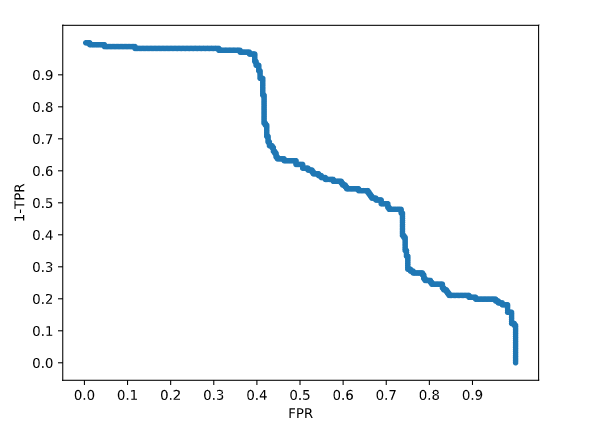
\includegraphics[width=1.0\textwidth]{rocCurve.png}
\end{figure}
\end{column}
\end{columns}
\end{frame}

\begin{frame}
\frametitle{Hog算法实现}
\begin{columns}
\begin{column}{.3\linewidth}
\begin{itemize}
	\item 依照\textbf{CVPR. 2005.177}实现Hog算法。
\end{itemize}
\end{column}
\begin{column}{.7\linewidth}
\begin{figure}[htbp]
	\centering
	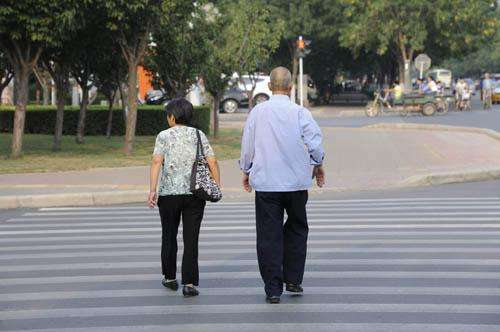
\includegraphics[width=0.6\textwidth]{example.jpg}
\end{figure}
\begin{figure}[htbp]
	\centering
	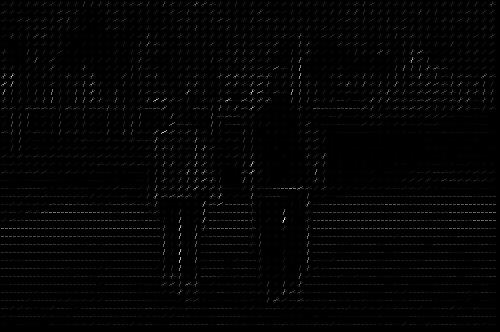
\includegraphics[width=0.6\textwidth]{example-hog.jpg}
\end{figure}
\end{column}
\end{columns}
\end{frame}

\begin{frame}
\frametitle{Hog Binary Classifier}
\begin{enumerate}
	\item Thanks for listening!
	\item Q\&A
\end{enumerate}
\end{frame}

\end{document}